\documentclass[tikz,border=8pt]{standalone}

\usepackage[T1]{fontenc}
\usepackage{lmodern}
\usepackage{amsmath,amssymb}
\usetikzlibrary{
  arrows.meta,
  calc,
  fit,
  positioning,
  backgrounds
}

\definecolor{featureblue}{RGB}{46,95,160}
\definecolor{latentgreen}{RGB}{45,125,92}
\definecolor{supervisionred}{RGB}{168,68,55}
\definecolor{trainfill}{RGB}{255,248,235}
\definecolor{retrievalfill}{RGB}{238,247,255}
\definecolor{linegray}{RGB}{70,70,70}

\tikzset{
  >=Latex,
  font=\sffamily,
  box/.style={
    draw=linegray,
    rounded corners=2pt,
    very thick,
    align=center,
    inner xsep=7pt,
    inner ysep=6pt,
    fill=white
  },
  smallbox/.style={
    box,
    font=\sffamily\small
  },
  tensor/.style={
    box,
    draw=featureblue,
    fill=featureblue!7,
    minimum width=36mm
  },
  latent/.style={
    box,
    draw=latentgreen,
    fill=latentgreen!8,
    minimum width=30mm
  },
  supervis/.style={
    box,
    draw=supervisionred,
    fill=supervisionred!8,
    minimum width=38mm
  },
  arrow/.style={
    ->,
    very thick,
    draw=linegray
  },
  shared/.style={
    ->,
    very thick,
    draw=featureblue
  },
  lossarrow/.style={
    ->,
    very thick,
    draw=supervisionred
  },
  retrievalarrow/.style={
    ->,
    very thick,
    draw=latentgreen
  },
  note/.style={
    align=left,
    font=\sffamily\footnotesize,
    text=linegray
  },
  title/.style={
    font=\sffamily\bfseries,
    align=center
  }
}

\begin{document}
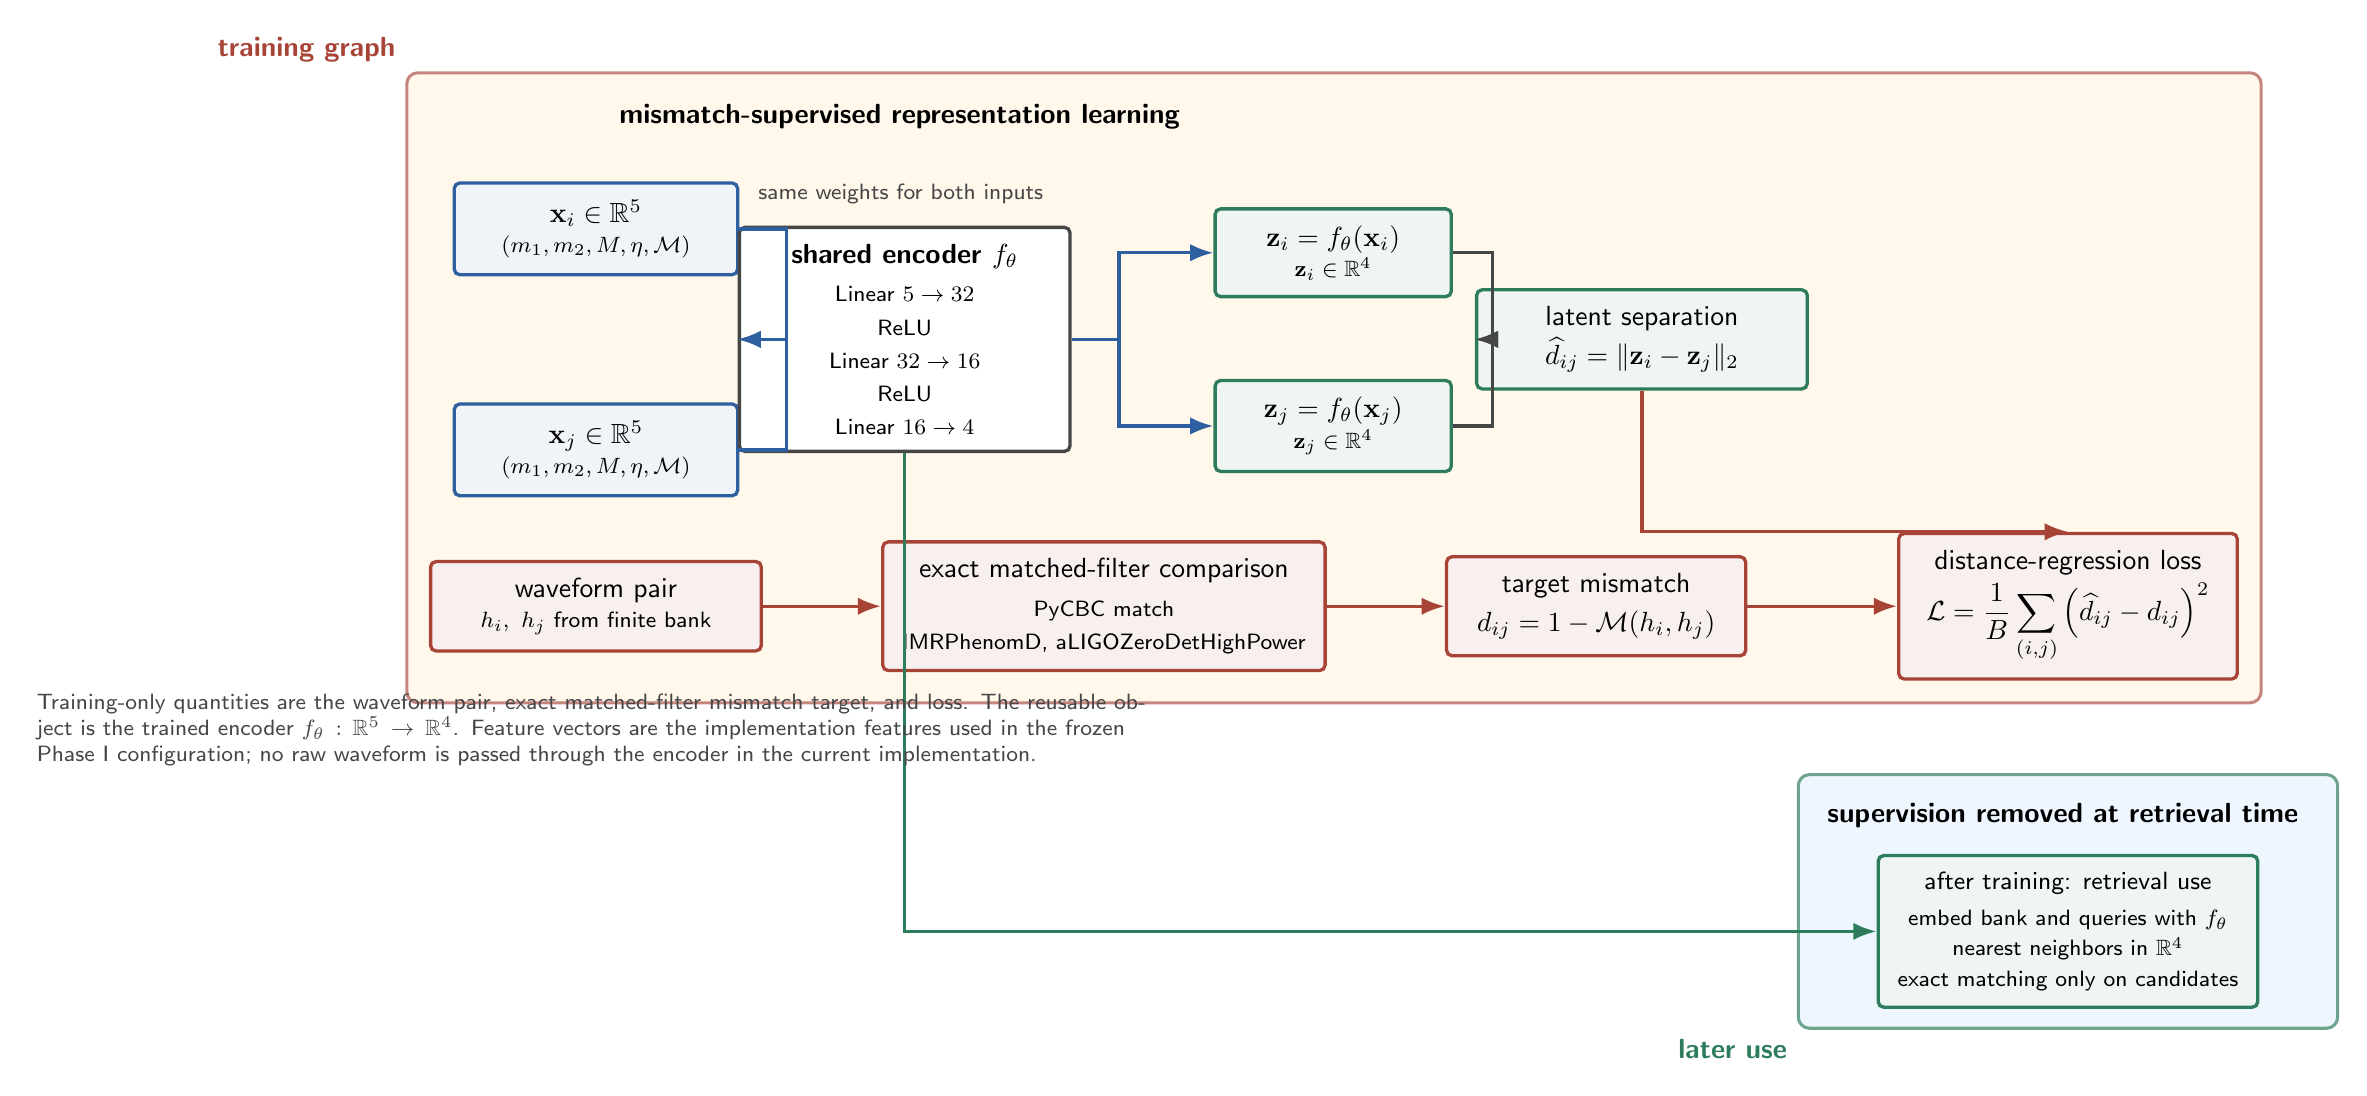
\begin{tikzpicture}[node distance=10mm and 14mm]

% Training inputs.
\node[tensor] (xi) {
  $\mathbf{x}_i \in \mathbb{R}^{5}$\\[-1pt]
  \footnotesize $(m_1,m_2,M,\eta,\mathcal{M})$
};
\node[tensor, below=16mm of xi] (xj) {
  $\mathbf{x}_j \in \mathbb{R}^{5}$\\[-1pt]
  \footnotesize $(m_1,m_2,M,\eta,\mathcal{M})$
};

% Shared encoder.
\node[box, right=18mm of $(xi)!0.5!(xj)$, minimum width=42mm] (encoder) {
  \textbf{shared encoder }$f_\theta$\\[2pt]
  \footnotesize Linear $5 \rightarrow 32$\\
  \footnotesize ReLU\\
  \footnotesize Linear $32 \rightarrow 16$\\
  \footnotesize ReLU\\
  \footnotesize Linear $16 \rightarrow 4$
};
\node[note, above=1.5mm of encoder] (sharednote) {
  same weights for both inputs
};

% Latent outputs.
\node[latent, right=18mm of encoder, yshift=11mm] (zi) {
  $\mathbf{z}_i=f_\theta(\mathbf{x}_i)$\\[-1pt]
  \footnotesize $\mathbf{z}_i \in \mathbb{R}^{4}$
};
\node[latent, right=18mm of encoder, yshift=-11mm] (zj) {
  $\mathbf{z}_j=f_\theta(\mathbf{x}_j)$\\[-1pt]
  \footnotesize $\mathbf{z}_j \in \mathbb{R}^{4}$
};

\node[latent, right=18mm of $(zi)!0.5!(zj)$, minimum width=42mm] (latentdist) {
  latent separation\\[2pt]
  $\widehat{d}_{ij}=\|\mathbf{z}_i-\mathbf{z}_j\|_2$
};

% Supervision branch.
\node[supervis, below=28mm of $(xi)!0.5!(xj)$, minimum width=42mm] (waveforms) {
  waveform pair\\[-1pt]
  \footnotesize $h_i,\ h_j$ from finite bank
};
\node[supervis, right=15mm of waveforms, minimum width=48mm] (match) {
  exact matched-filter comparison\\[2pt]
  \footnotesize PyCBC match\\
  \footnotesize IMRPhenomD,\ aLIGOZeroDetHighPower
};
\node[supervis, right=15mm of match, minimum width=38mm] (mismatch) {
  target mismatch\\[2pt]
  $d_{ij}=1-\mathcal{M}(h_i,h_j)$
};

% Loss.
\node[supervis, right=19mm of mismatch, minimum width=43mm] (loss) {
  distance-regression loss\\[2pt]
  $\displaystyle
    \mathcal{L}
    =\frac{1}{B}\sum_{(i,j)}
    \left(\widehat{d}_{ij}-d_{ij}\right)^2$
};

% Retrieval use after training.
\node[smallbox, below=22mm of loss, draw=latentgreen, fill=latentgreen!8, minimum width=45mm] (retrieval) {
  after training: retrieval use\\[2pt]
  \footnotesize embed bank and queries with $f_\theta$\\
  \footnotesize nearest neighbors in $\mathbb{R}^{4}$\\
  \footnotesize exact matching only on candidates
};

% Main arrows.
\draw[shared] (xi.east) -- ++(6mm,0) |- (encoder.west);
\draw[shared] (xj.east) -- ++(6mm,0) |- (encoder.west);
\draw[shared] (encoder.east) -- ++(6mm,0) |- (zi.west);
\draw[shared] (encoder.east) -- ++(6mm,0) |- (zj.west);
\draw[arrow] (zi.east) -- ++(5mm,0) |- (latentdist.west);
\draw[arrow] (zj.east) -- ++(5mm,0) |- (latentdist.west);

\draw[lossarrow] (waveforms.east) -- (match.west);
\draw[lossarrow] (match.east) -- (mismatch.west);
\draw[lossarrow] (mismatch.east) -- (loss.west);
\draw[lossarrow] (latentdist.south) |- (loss.north);

\draw[retrievalarrow] (encoder.south) |- (retrieval.west);

% Labels distinguishing training and retrieval.
\node[title, above=11mm of encoder] (traintitle) {
  mismatch-supervised representation learning
};
\node[title, above=2mm of retrieval] (retrievaltitle) {
  supervision removed at retrieval time
};

\node[note, below=4mm of waveforms, text width=142mm] (footnote) {
  Training-only quantities are the waveform pair, exact matched-filter mismatch
  target, and loss. The reusable object is the trained encoder
  $f_\theta:\mathbb{R}^{5}\rightarrow\mathbb{R}^{4}$. Feature vectors are the
  implementation features used in the frozen Phase I configuration; no raw
  waveform is passed through the encoder in the current implementation.
};

% Background grouping.
\begin{scope}[on background layer]
  \node[
    draw=supervisionred!65,
    fill=trainfill,
    rounded corners=4pt,
    line width=1.1pt,
    fit=(xi)(xj)(encoder)(zi)(zj)(latentdist)(waveforms)(match)(mismatch)(loss)(traintitle),
    inner sep=8pt,
    label={[font=\sffamily\bfseries, text=supervisionred]north west:training graph}
  ] {};
  \node[
    draw=latentgreen!70,
    fill=retrievalfill,
    rounded corners=4pt,
    line width=1.1pt,
    fit=(retrieval)(retrievaltitle),
    inner sep=7pt,
    label={[font=\sffamily\bfseries, text=latentgreen]south west:later use}
  ] {};
\end{scope}

\end{tikzpicture}
\end{document}
